%%%%%%%%%%%%%%%%%%%%%%%%%%%%%%%%%%%%%%%%%
% University Assignment Title Page 
% LaTeX Template
% Version 1.0 (27/12/12)
%
% This template has been downloaded from:
% http://www.LaTeXTemplates.com
%
% Original author:
% WikiBooks (http://en.wikibooks.org/wiki/LaTeX/Title_Creation)
%
% License:
% CC BY-NC-SA 3.0 (http://creativecommons.org/licenses/by-nc-sa/3.0/)
% 
% Instructions for using this template:
% This title page is capable of being compiled as is. This is not useful for 
% including it in another document. To do this, you have two options: 
%
% 1) Copy/paste everything between \begin{document} and \end{document} 
% starting at \begin{titlepage} and paste this into another LaTeX file where you 
% want your title page.
% OR
% 2) Remove everything outside the \begin{titlepage} and \end{titlepage} and 
% move this file to the same directory as the LaTeX file you wish to add it to. 
% Then add \input{./title_page_1.tex} to your LaTeX file where you want your
% title page.
%
%%%%%%%%%%%%%%%%%%%%%%%%%%%%%%%%%%%%%%%%%
%\title{Title page with logo}
%----------------------------------------------------------------------------------------
%	PACKAGES AND OTHER DOCUMENT CONFIGURATIONS
%----------------------------------------------------------------------------------------


\documentclass[12pt]{article}
\usepackage{gensymb}
\usepackage[spanish]{babel}
\usepackage[utf8x]{inputenc}
\usepackage{amsmath}
\usepackage{amssymb}
\usepackage{graphicx}
\usepackage{hyperref}
\usepackage{physics}
\usepackage{esvect}
\usepackage{esint}
\usepackage{comment}
\usepackage[colorinlistoftodos]{todonotes}
\usepackage{float}
\usepackage{multirow}
\usepackage{amsthm}


\usepackage{subfig}
\usepackage{svg}
\usepackage[a4paper]{geometry}
\usepackage{changepage}


%\def\dbar{{\mathchar’26\mkern-12mu d}}
\newcommand{\dbar}{\mathchar'26\mkern-12mu d}
\newtheorem{defi}{ Definición}[section]
\newtheorem{prep}{ Proposición}[section]
\newtheorem{teo}{ Teorema}[section]
\newtheorem{cor}{ Corolario}[section]
\newtheorem{lema}{Lema}[section]
\newtheorem{ejem}{Ejemplos}[section]





%\setpapersize{A4}
\begin{comment}
%\usepackage{vmargin} Paquete incompatible com geometry
\setmargins{2.5cm}       % margen izquierdo
{1.5cm}                        % margen superior
{16cm}                      % anchura del texto
{23.42cm}                    % altura del texto
{10pt}                           % altura de los encabezados
{1cm}                           % espacio entre el texto y los encabezados
{0pt}                             % altura del pie de página
{2cm}                           % espacio entre el texto y el pie de página
\end{comment}

\newgeometry{left=2.5cm,top=2.5cm,width=16cm,height=23.42cm,head=3.5mm,headsep=1cm,foot=1cm,bottom=3cm}

\savegeometry{standard}



\begin{document}

\begin{titlepage}

\newcommand{\HRule}{\rule{\linewidth}{0.5mm}} % Defines a new command for the horizontal lines, change thickness here

\center % Center everything on the page
 
%----------------------------------------------------------------------------------------
%	HEADING SECTIONS
%----------------------------------------------------------------------------------------
\textsc{\LARGE Universidad de Granada}\\[1.5cm] % Name of your university/college
\textsc{\Large Física del estado sólido}\\[0.5cm] % Major heading such as course name
\textsc{\large Doble Grado en Física y Matemáticas}\\[0.5cm] % Minor heading such as course title

%----------------------------------------------------------------------------------------
%	TITLE SECTION
%----------------------------------------------------------------------------------------

\HRule \\[0.4cm]
{ \huge \bfseries AED en variables sobre Estados.}\\[0.2cm] % Title of your document
\HRule \\[1cm]
 
%----------------------------------------------------------------------------------------
%	AUTHOR SECTION
%----------------------------------------------------------------------------------------

% If you don't want a supervisor, uncomment the two lines below and remove the section above
% Your name

%----------------------------------------------------------------------------------------
%	DATE SECTION
%----------------------------------------------------------------------------------------

%{\large 7 de Abril de  2021}\\[1cm] % Date, change the \today to a set date if you want to be precise

%----------------------------------------------------------------------------------------
%	LOGO SECTION
%----------------------------------------------------------------------------------------


\includegraphics[width=0.7\textwidth]{UGR-Logo.png}\\[1.5cm] % Include a department/university logo - this will require the graphicx package
\textsc{\large Aarón Benitez Barón}\\[0.5cm]


 
%----------------------------------------------------------------------------------------

\vfill % Fill the rest of the page with whitespace

\end{titlepage}

\tableofcontents
\newpage

\begin{centering}
\section*{Abstract}
En este informe se recoge el estudio estadístico de distintas variables demográficas recogidas sobre países del mundo. Estudiaremos supuestos de normalidad de las variables con el objetivo de poder aplicar técnicas de reducción de la dimensión a estos datos.
Por último intentaremos obtener un modelo mediante análisis discriminante si un país esta desarrollado o no.
\end{centering}

\section{Introducción}
La reducción de dimensión es una técnica muy útil en el campo del machine learning ya que este permite reducir el tamaño de memoria que consumen los datos, el tiempo operacional y la mejora de la visualización de las variables. En esta práctica aplicaremos distintos métodos como el Análisis de Componentes Principales o el Análisis Factorial para llevar a cabo esta técnica.
Después de ello intentaremos aplicar una técnica muy conocida en el reconocimiento de patrones como es el Análisis de Discriminante para discernir propiedades de la base de datos elegida.
En nuestro caso, estudiaremos datos demográficos sobre 34 países distintos que nos darán información sobre la situación de desarrollo del Estado. Dichas variables las expondremos en el siguiente apartado.
El objetivo será tratar la base de datos que nos den, tratar con sus ouliers, valores perdidos, etc. y a partir de ahí, estudiar tanto el comportamiento de las variables por separado como sus correlaciones que nos permitan aplicar las técnica del análisis estadístico multivariante.

\section{Materiales y métodos}

\subsection{Materiales}
En este apartado, presentaremos la base de datos a estudiar. Estudiaremos 11 variables distintas que serán:
\begin{itemize}
\item Densidad de población.
\item Población en núcleos urbanos.
\item Población trabajando en el sector agrícola.
\item Población trabajando en el sector servicio.
\item Coeficiente entre población activa y total.
\item Esperanza de vida.
\item Tasa de mortalidad infantil.
\item Tasa entre el número de individuos en ejército de tierra y población total.
\item Tasa de médicos por habitante.
\item Número de libro publicados.
\item Tasa de consumo energéico.
\end{itemize}

Todas estas variables están normalizadas debido a las distintas unidades que puedan tener. A continuación, presentamos una tabla que expone los diferentes estadísticos más relevantes sobre estas variables:

\begin{table}[H]
\begin{centering}
\begin{tabular}{|c|c|c|}
\hline 
 & Centrimedia & CVc\tabularnewline
\hline 
\hline 
Densidad población & -0.2293829 & -4.7611940\tabularnewline
\hline 
Población urbana & 0.1147624 & 18.6903015\tabularnewline
\hline 
Población agricola & -0.20433276 & -11.4243309\tabularnewline
\hline 
Población servicio & 0.00064957 & 12.8296875\tabularnewline
\hline 
Población activa & 0.02917055 & 7.5584589\tabularnewline
\hline 
Esperanza de vida & 0.17613181 & 10.4877506\tabularnewline
\hline 
Mortalidad infantil & -0.2268480 & -30.8993711\tabularnewline
\hline 
Tasa de militares & -0.2192510 & -1.3081800\tabularnewline
\hline 
Tasa de médicos & -0.149734266 & -130.4526316\tabularnewline
\hline 
Libros publicados & -0.2615358 & -7.2311230\tabularnewline
\hline 
Consumo energético & -0.26271176 & -6.871948\tabularnewline
\hline 
\end{tabular}
\par\end{centering}
\caption{Valores de centralidad y coeficientes de variación cuartílica para
las distintas variables.}
He decidido usar estas medidas de centralidad y dispersión porque son mucho más significativas para estas variables que las usuales media y desviación típica.
\end{table}

\subsection{Métodos}
En esta sección presentaremos las técnicas que vamos a utilizar para estudiar estas variables:
\begin{itemize}
\item En primer lugar, estudiaremos la normalidad univariante de cada variable a través de gráficos qq-plot.
\item A continuación, comprobaremos que realmente existen correlaciones entre las variables con un test de Barlett.
\item Aplicaremos el Análisis de Componentes principales, con diferentes métodos para decidir cuantas componentes tomar.
\item También aplicaremos un Análisis Factorial mediante el modelo varimax para obtener las variables latentes en los datos.
\item Por último aplicaremos un Análisis Discriminante lineal y cuadrático con el cuál seremos capaces de predecir si un país dado es desarrollado o no.

\end{itemize}

\section{Resultados}
Una vez tratada la base de datos, eliminando los outliers y los valores perdidos pertinentes, procedemos a desarrollar los resultados.
\subsection{Normalidad univariante}
Comprobemos en primer lugar si las variables por separado siguen aproximadamente un comportamiento normal. Para ello utilizaremos un qq-plot:

\begin{figure}[H]
    \centering
    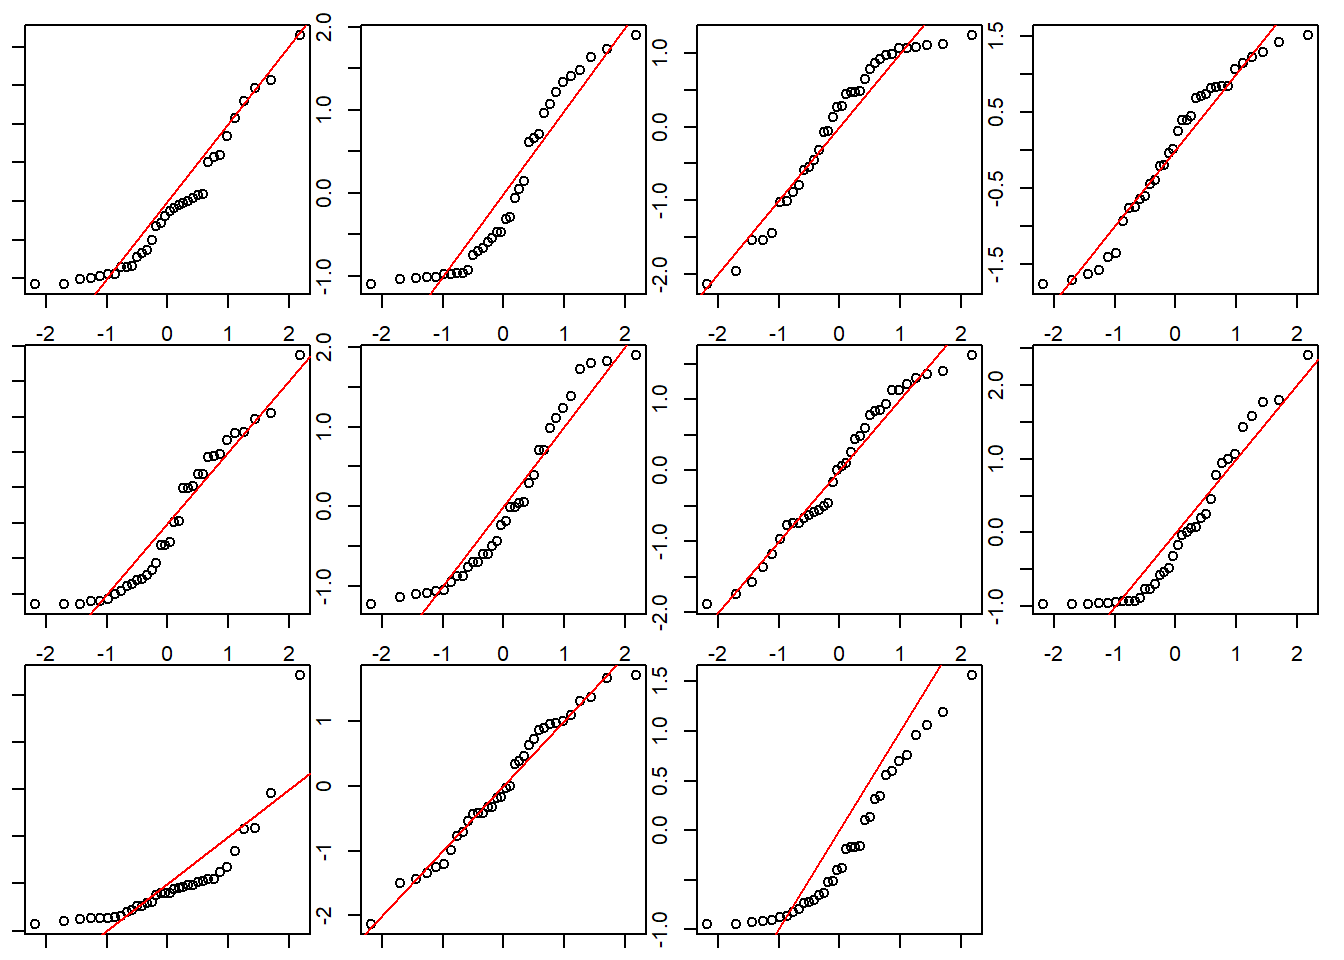
\includegraphics[scale=1]{qq-plot.png}
    \caption{Estudio de la normalidad de las variables.}
\end{figure}

Observamos que en general, nuestras variables se desvían del comportamiento normal. Sin embargo, como no es una desviación muy extrema (salvo en la variable 9, correspondiente a la tasa de militares) asumiremos normalidad en dichas variables. 

\subsection{Test de Barlett}
Si representamos la matriz de correlaciones de forma gráfica obtenemos el siguiente resultado:
\begin{figure}[H]
    \centering
    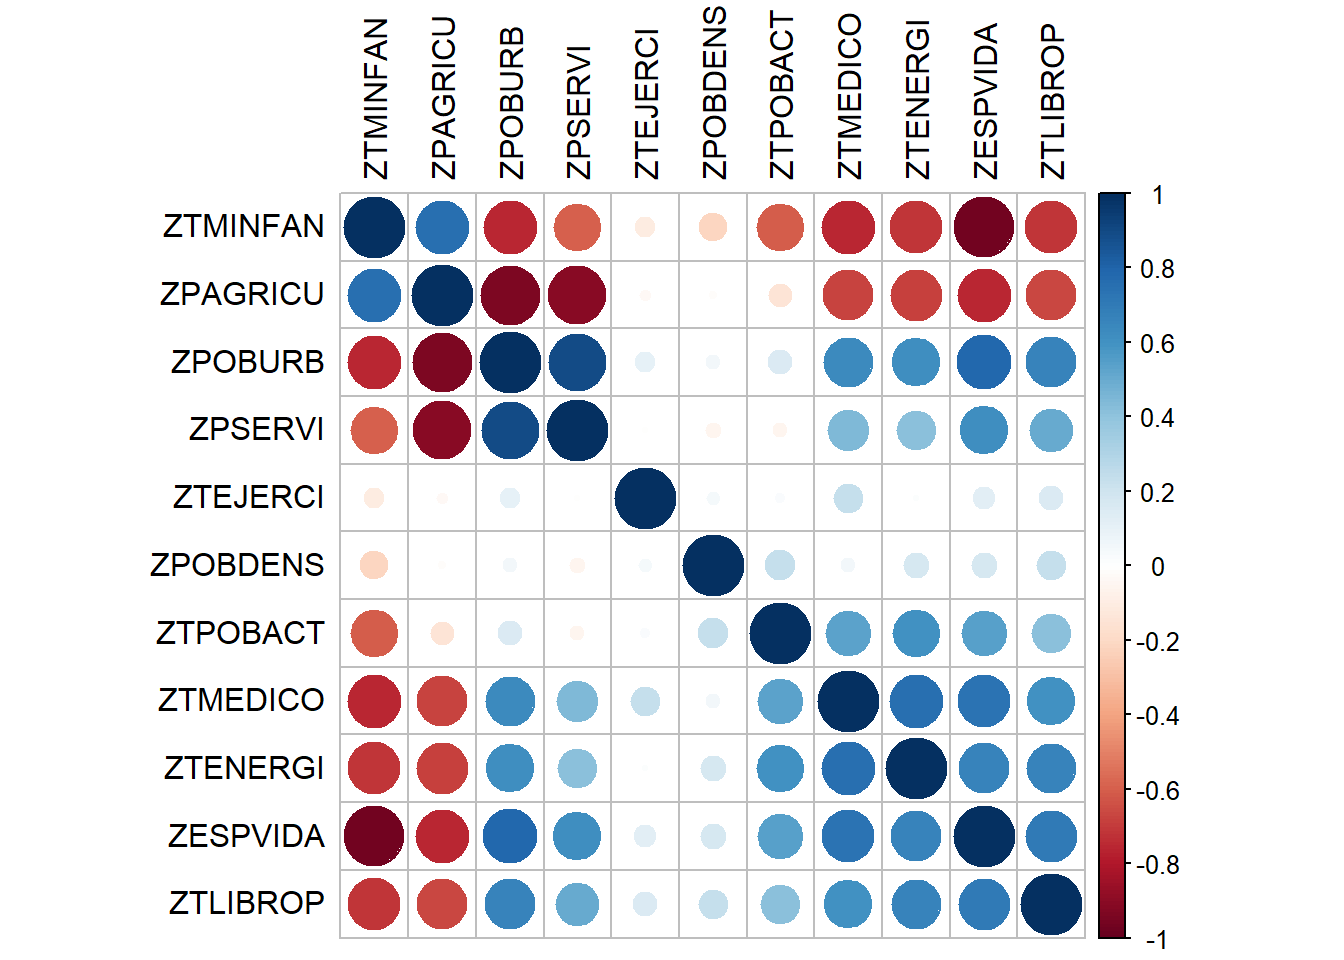
\includegraphics[scale=0.8]{correl.png}
    \caption{Estudio de la normalidad de las variables.}
\end{figure}
Observamos que claramente existen correlaciones entre las variables, sin embargo realizamos el test de Barlett para asegurarnos de ello. En el obtuvimos un p-valor muy cercano a cero, por lo que tenemos que rechazar la hipótesis nula $H_0$ y aseguramos que la matriz de correlaciones no es trivial.

\subsection{Análisis de Componentes principales.}

A continuación aplicaremos el método de las componentes principales. Para obtener el número de componentes que debemos considerar utilizaremos varios métodos. En primer lugar, presentamos el método del codo:

\begin{figure}[H]
    \centering
    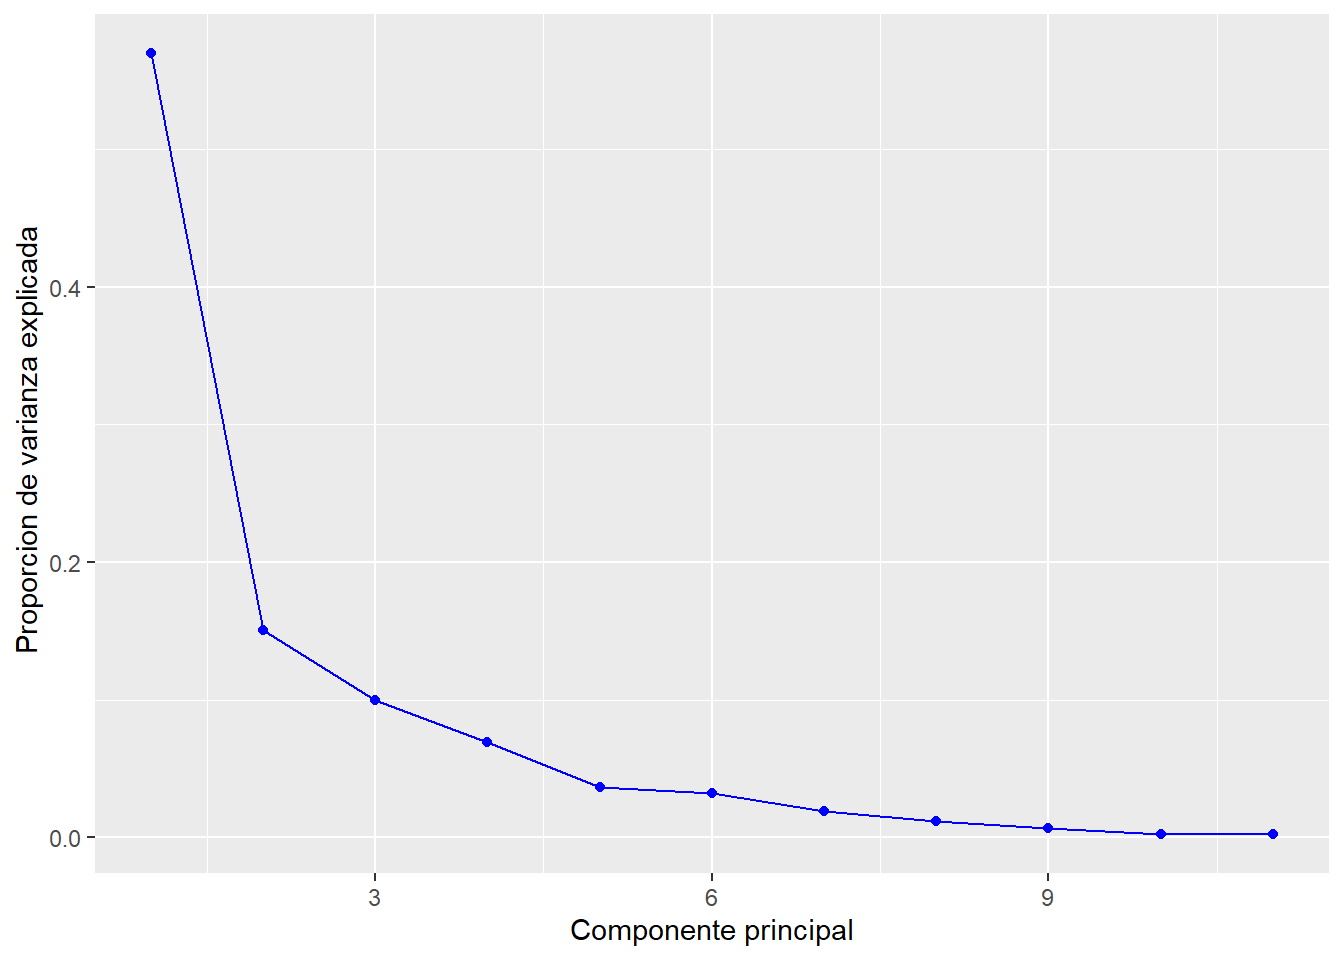
\includegraphics[scale=0.8]{codo.png}
    \caption{Gráfico de la varianza explicada de cada CP.}
\end{figure}

Observamos que el codo nos dice que tomemos 2 componentes principales. Sin embargo, los métodos de la varianza acumulada y la Regla de Abdi nos "aconsejan" que tomemos 3. La decisión final será tomar tres componentes para cubrir más del 80$\%$ de la varianza explicada. Las componentes principales quedan así:

\begin{figure}[H]
    \centering
    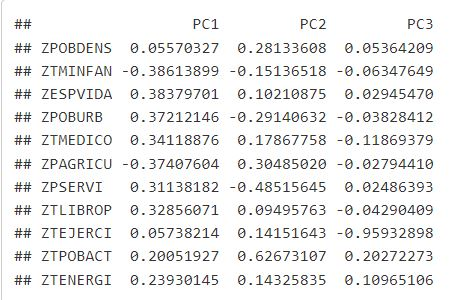
\includegraphics[scale=0.8]{PCA.JPG}
    \caption{Resultado de las componentes principales.}
\end{figure}
Si representamos las contribuciones de cada variable a las componentes obtenemos los siguientes gráficos:
\begin{figure}[H]
    \centering
    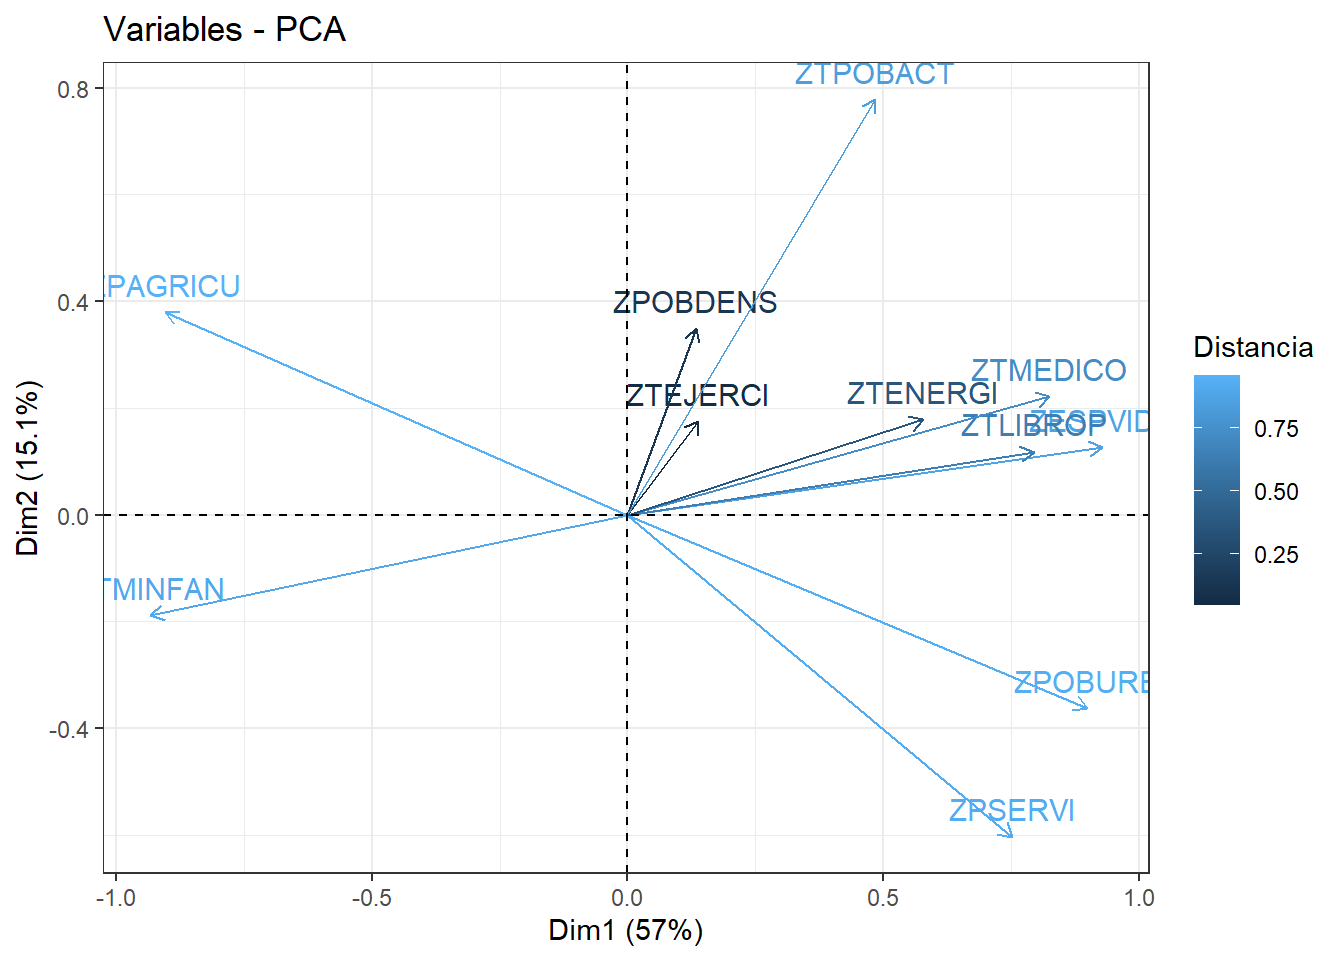
\includegraphics[scale=0.4]{cp1.png}
    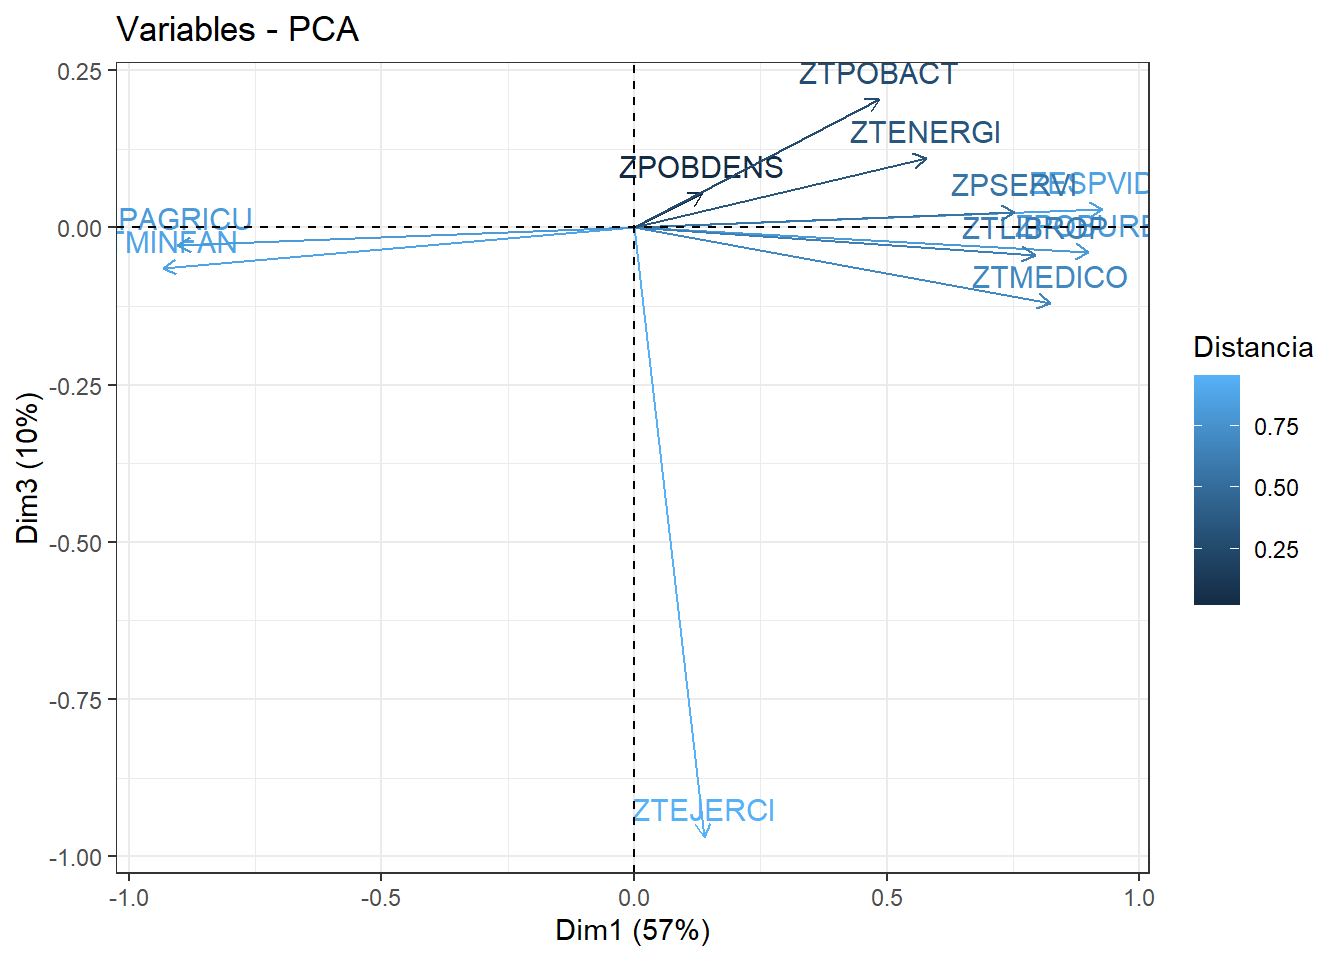
\includegraphics[scale=0.4]{cp2.png}
    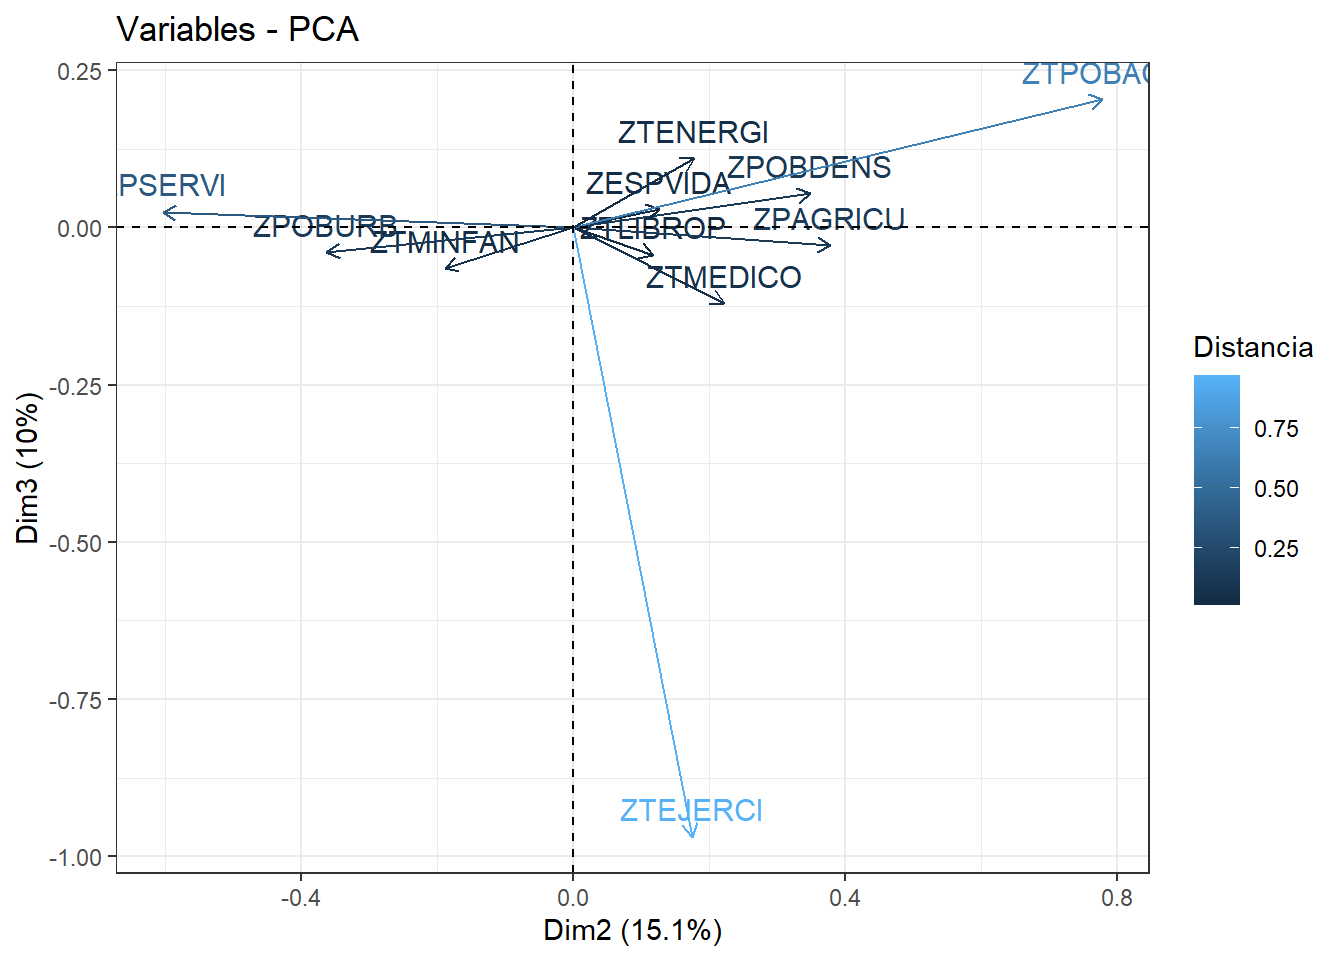
\includegraphics[scale=0.4]{cp3.png}
    \caption{Representación de las contribuciones para cada compoenente principal.}
\end{figure}

\subsection{Análisis Factorial}
Antes de aplicar el modelo correspondiente para obtener los factores latentes, debemos discernir cuantos factores vamos a considerar. Para ello utilizaremos el análisis paralelo:
\begin{figure}[H]
    \centering
    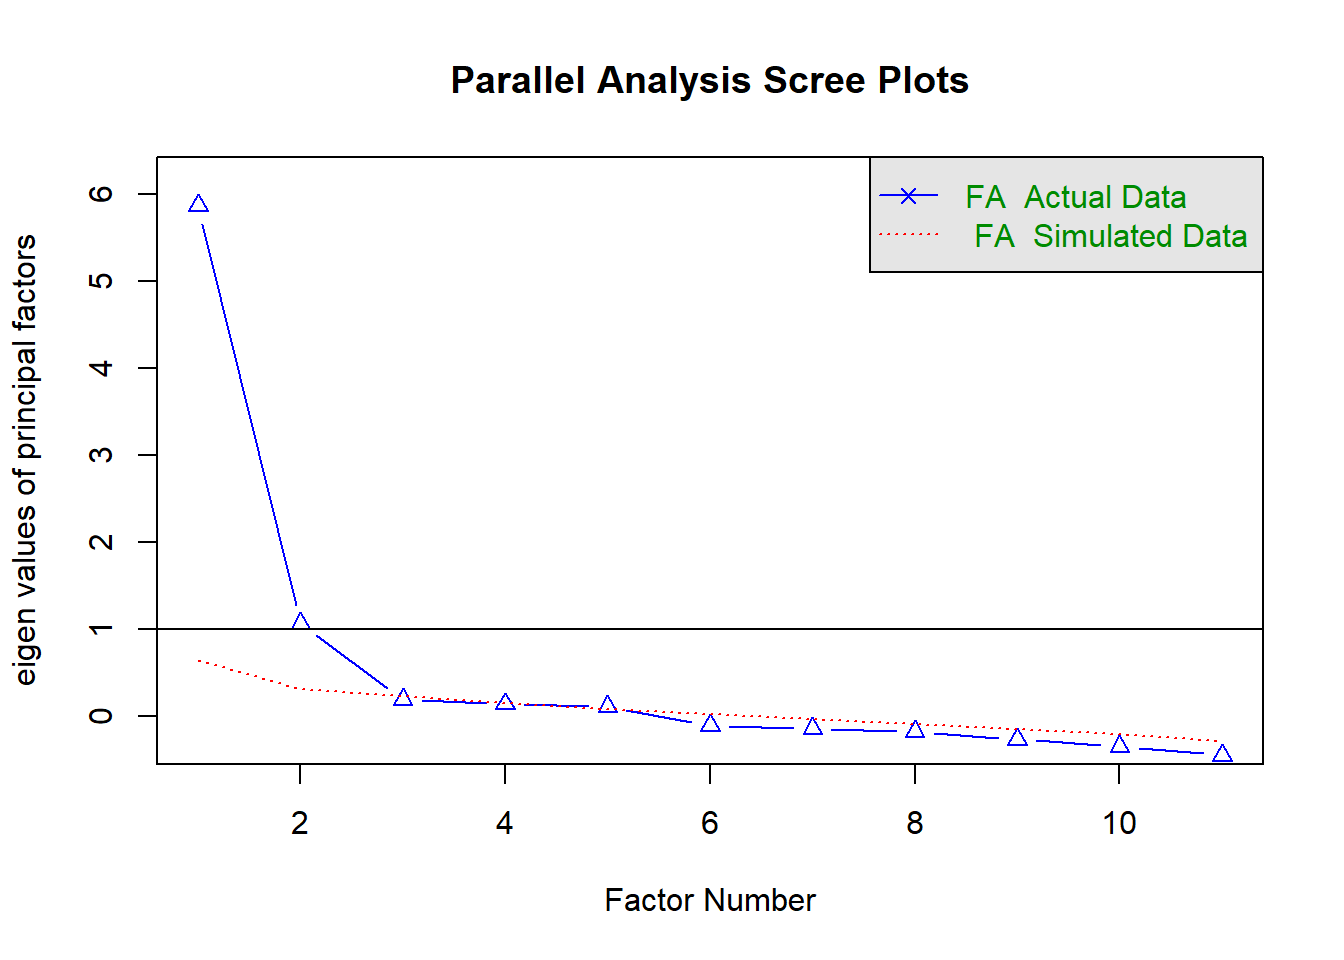
\includegraphics[scale=0.6]{paralelo.png}
    \caption{Gráfico del análisis paralelo.}
\end{figure}
En vistas de este, tomaremos 2 factores latentes. Aplicando el modelo varimax, obtenemos los siguientes factores:
\begin{figure}[H]
    \centering
    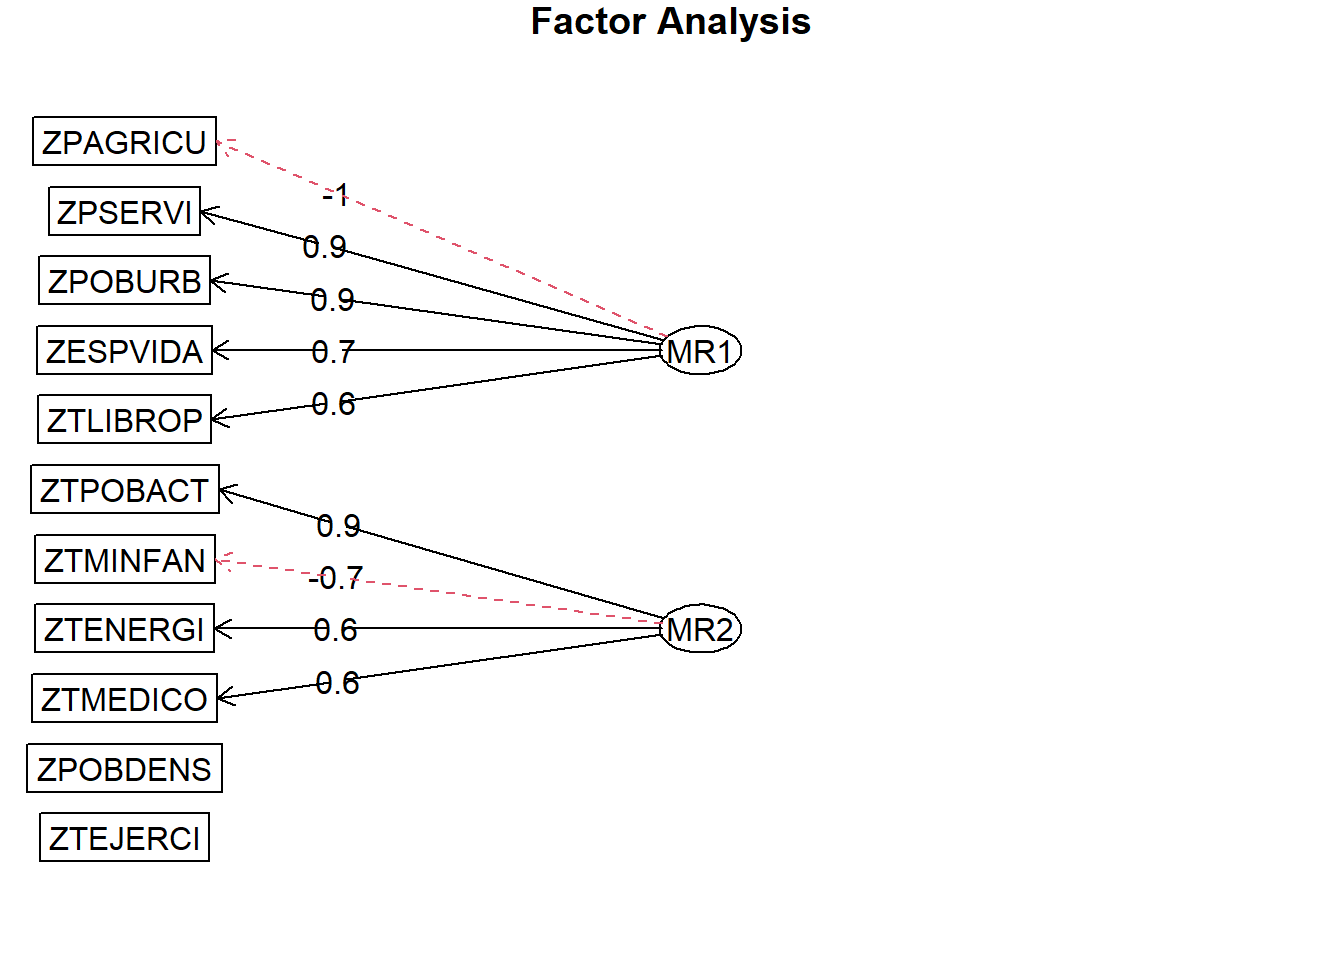
\includegraphics[scale=0.6]{factores.png}
    \caption{Diagrama de factores latentes.}
\end{figure}

\subsection{Análisis Discriminante}
Antes de aplicar este método, estudiaremos el supuesto de normal multivariante a través de distintos test, como el de Royston y el de Henze-Zirkler. Si realizamos, el test con todas las variables, obtenemos que la negación de este hecho. Sin embargo, al eliminar la variable que recogía la tasa de militares (ya que esta se alejaba demasiado del comportamiento normal) si obtenemos normalidad con el test de Henze-Zirkler. Con esto nos bastará para aplicar el método.
El objetivo de este análisis será ser capaces de dilucidar si un país es desarrollado o subdesarrollado según los datos dados.
El análisis discriminante lineal nos da casi un 15$\%$ de error al contrastarlo con la matriz de confusión, sin embargo, el cuadrático nos da una tasa de error del 0$\%$ por lo que será este el que realmente tendremos en cuenta. Los resultados de dicho análisis fueron:

\begin{figure}[H]
    \centering
    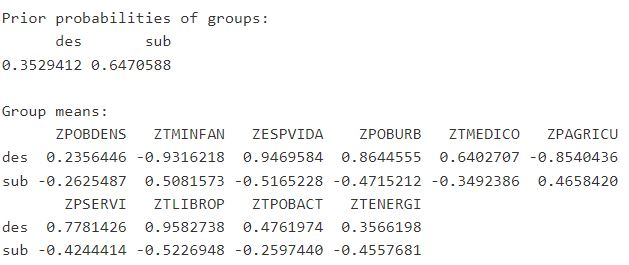
\includegraphics[scale=0.8]{ADC.JPG}
    \caption{Resultado del análisis discriminante cuadrático.}
\end{figure}
Observamos que a priori, la probabilidad de que un pais sea desarrollado es de solamente un 35$\%$. Si representamos algunas variables que relaciona nuestro análisis, vemos como este consigue clasificar los países como se pretendía;
\begin{figure}[H]
    \centering
    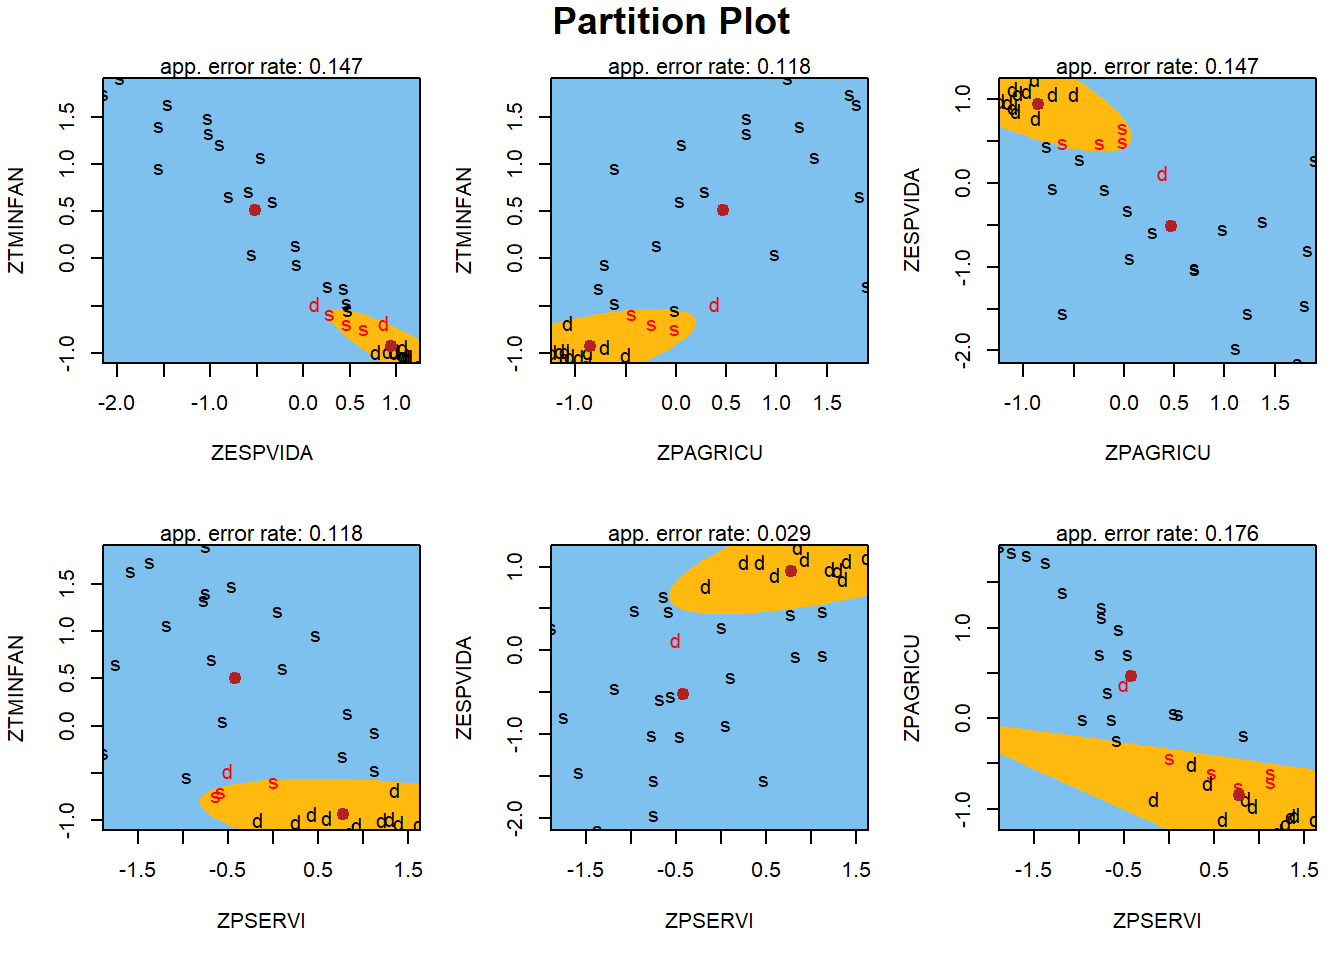
\includegraphics[scale=0.8]{adimage.png}
    \caption{Gráficos de clasificación para el análisis discriminante.}
\end{figure}

\section{Discusión}
Vamos a interpretar un poco los resultados obtenidos. Cabe destacar que los supuestos de normalidad, tanto univariante como multivariante no son para nada robustos, por lo que no podemos asegurar con autoridad de que los resultados obtenidos sean completamente correctos.
Obviando esto hemos conseguido reducir la dimensión de la muestra como se pretendía con el ACP y el AF. Cabe destacar la interpretación que le podemos dar a los factores latentes obtenidos:
\begin{itemize}
\item El MF1 podría darnos un indicador de como de urbanizado esta un país, teniendo en cuenta positivamente las variables de personas trabajando en sector servicio y la población residente en ciudades, además de valorar negativamente la población agrícola. Con menos fuerza también valora positivamente la esperanza de vida y la cantidad de libros publicados.
\item El MF2 nos da idea de un desarrollo más general del país, valorando si se dan ciertas necesidades básicas. En este factor se recoge positivamente si hay pocos parados, la tasa de médicos y la energía que se consume. Por último, se valora negativamente la mortalidad infantil en el país. Este indicador podría ser útil para compara países en vías de desarrollo.
\end{itemize}
Por último, en el análisis Discriminante se han conseguido resultados fructíferos a la hora de hacer una clasificación entre los distintos países, por lo menos si aplicábamos el modelo cuadrático, dando a entender que las relaciones son algo más complejas como para tratarlas únicamente con un modelo lineal.

\section{Conclusión}
Pese a la limitación de conocimiento por mi parte, creo que se han conseguido resultados interesantes sobre las variables expuestas. Para mejorar el trabajo tendríamos que realmente comprobar si estos métodos son aplicables con los supuestos de normalidad que se han dado. También podríamos completar este informe estudiando muchas más variables demográficas que nos de información más rica para el estudio.
En conclusión, los objetivos que se establecían se han cumplido en gran medida por lo que podemos dar por cerrado este trabajo.
\end{document}
